%----------------------------------------------------------------------------
\chapter{Background}\label{ch:background}
%----------------------------------------------------------------------------

In this chapter I address the foundations of this work. In \autoref{sec:formalisms} I introduce the theoretical bases of behaviour modeling, which is used widely in systems engineering, and their implementation in an existing language - SysML. After this I talk about Formal Verification in \autoref{sec:formal_verification}, which is a mathematically rigorous method for finding specific configurations of modelled systems. Lastly, I introduce the Gamma Composite Statechart Framework, which is a tool for stating and verifying composite models using statechart behaviours.

%----------------------------------------------------------------------------
\section{Behaviour Models}\label{sec:behaviour_models}
%----------------------------------------------------------------------------

\subsection{Finite State Machine}

Finite state machines (FSMs) are widely used formalisms to model computation. They can be in exactly one of a finite number of \emph{states} at any given time. FSM can change from one state to another in response to some \emph{inputs} (usually called signals); which change is called a \emph{transition} (see \autoref{fig:fsm} for an example finite state machine).

\begin{figure}[!ht]
	\centering
	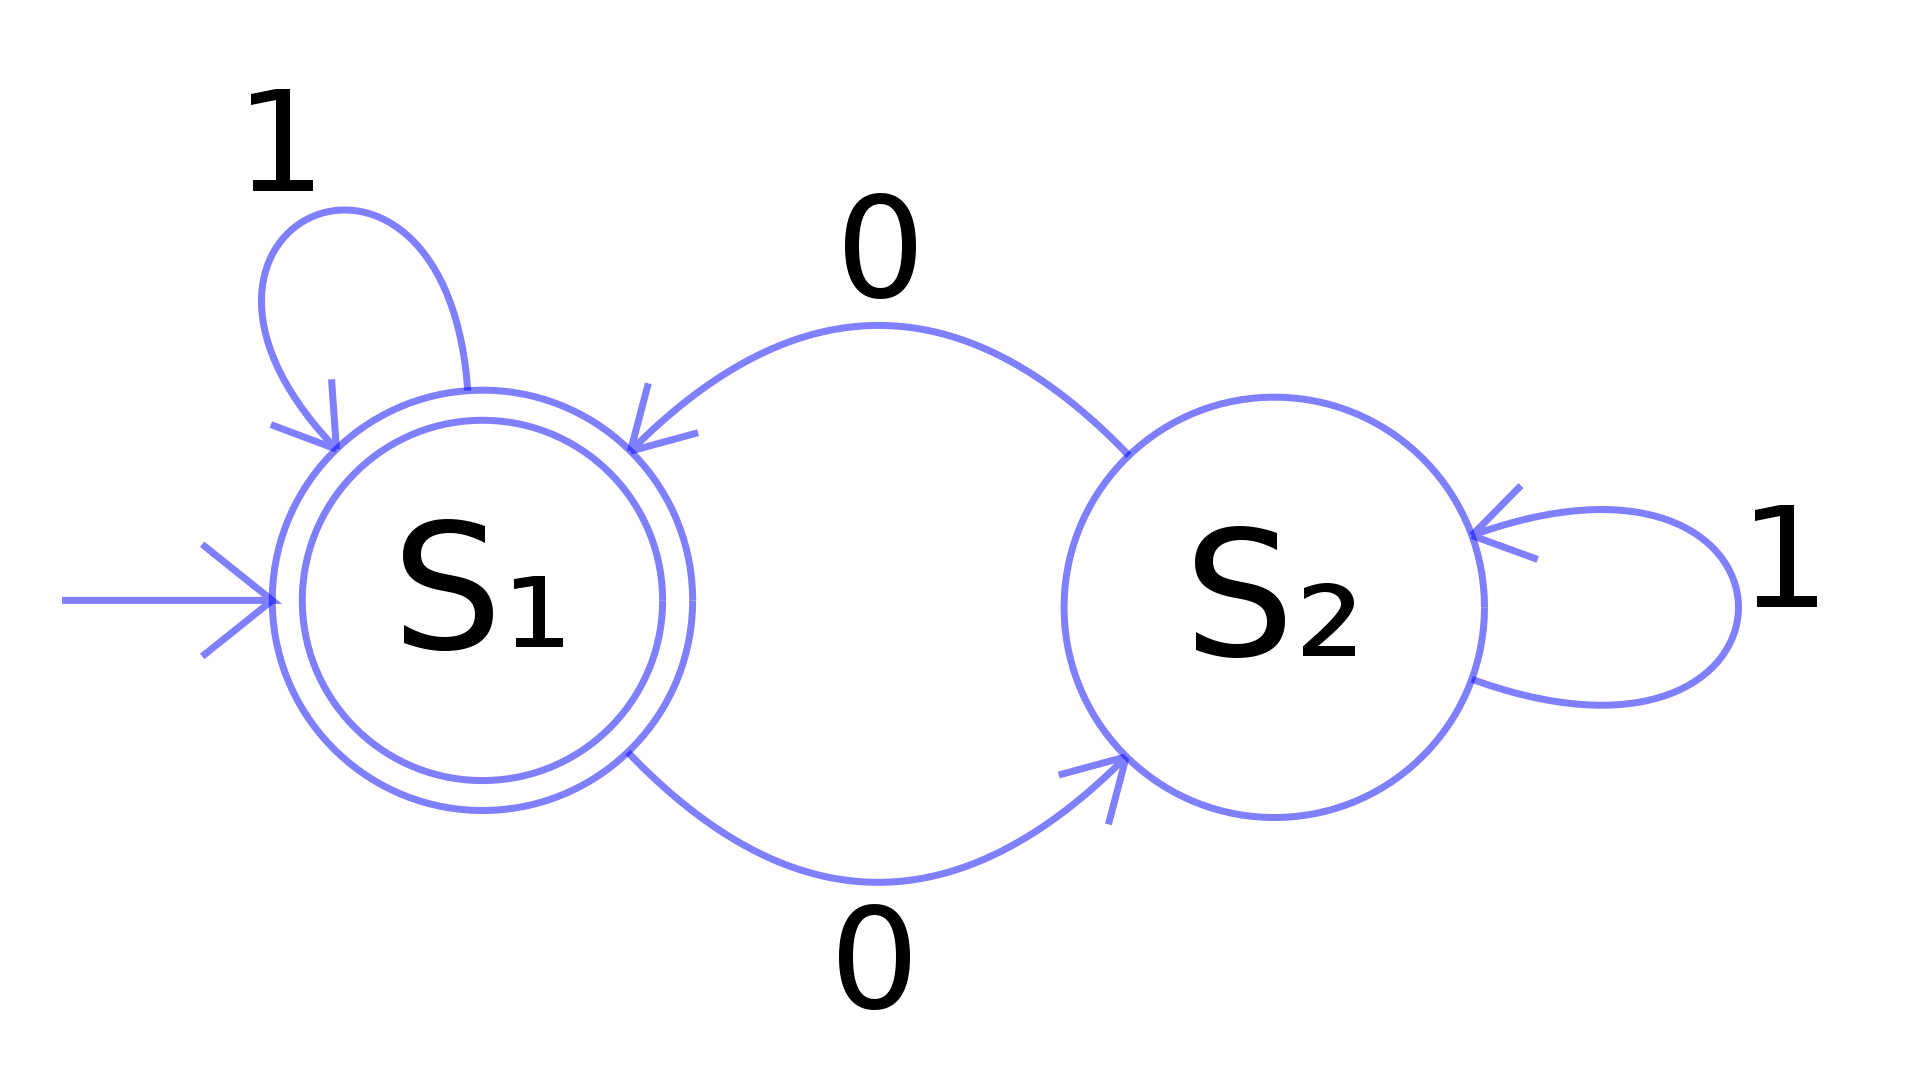
\includegraphics[width=67mm, keepaspectratio]{figures/fsm.png}\hspace{1cm}
	\caption{An example deterministic finite state machine, which checks a given binary numbers \emph{evenness}.}
	\label{fig:fsm}
\end{figure}

The formal definition of \emph{deterministic} finite state machines is as follows.

\begin{definition}[Deterministic finite state machine]
	
	A DFSM is a tuple \( SM = (\Sigma, S, s_0, \delta, F) \)
	
	\begin{itemize}
		\item \(\Sigma\) is the set input \emph{alphabet} (a finite non-empty set of symbols);
		\item \(S\) is a finite non-empty set of states;
		\item \(s_0 \in S\) is an initial state;
		\item \(\delta : S \times \Sigma \rightarrow S \) is the state-transition function;
		\item \(F \subseteq S\) is the set of final states
	\end{itemize}
\end{definition}

The current state of a DFSM is \(s \in S\). A transition from state to state is performed, given the last input letter \(l\), if and only if \( s' = \delta(s, l) \in S \). In which case the current state will become \(s'\) (this work assumes, that if the given \(\delta(s, l)\) is not defined, then the state machine remains in it's current state).

\subsection{Petri Net}

\begin{figure}[!ht]
	\centering
	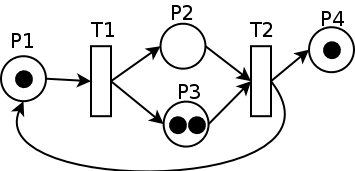
\includegraphics[width=67mm, keepaspectratio]{figures/petri_net.png}\hspace{1cm}
	\caption{An example Petri net with 2 transitions and 4 places.}
	\label{fig:petri_net}
\end{figure}

Petri nets are a widely used formalism to model concurrent, asynchronous systems \cite{24143}. The formal definition of a Petri net (including inhibitor arcs) is as follows (see \autoref{fig:petri_net} for an illustration of the notations).

\begin{definition}[Petri net]
	
	A Petri net is a tuple \( PN = (P, T, W, M_0) \)
	
	\begin{itemize}
		\item \(P\) is the set of \emph{places} (defining state variables);
		\item \(T\) is the set of \emph{transitions} (defining behaviour), such that \( P \bigcap T = \emptyset \);
		\item \(W \subseteq W^+ \bigcup W^- \) is a set of two types of arcs, where \(  W^+ : T \times P \rightarrow \mathbb{N}\) and \( W^- : P \times T \rightarrow \mathbb{N} \) are the set of input arcs and output arcs, respectively (\( \mathbb{N} \) is the set of all natural numbers);
		\item \(M_0 : P \rightarrow \mathbb{N} \) is the \emph{initial marking}, i.e., the number of \emph{tokens} on each place.
	\end{itemize}
\end{definition}

The state of a Petri net is defined by the current marking \( M : P \rightarrow \mathbb{N} \). The behaviour of the systems is described as follows. A transition \( t \) is enabled if \( \forall p \in P : M(p) \in W(p, t) \). Any enabled transition \(t\) may fire non-deterministically, creating the new marking \( M' \) of the Petri as follows: \( \forall p \in P : M'(p) = M(p) - W^-(p, t) + W^+(t, p) \).

In words: W describes the \emph{weight} of each flow from a transition to a place, or from a place to a transition. Firing a transition \(t\) in a marking \(M\) consumes \(W^-(p_i, t)\) tokens from each of its input places \(p_i\), and produces \(W(t, p_o)\) tokens in each of its output places \(p_o\). One such transition \(t\) is \emph{enabled} (it may \emph{fire}) in \(M\) if there are enough tokens in its input places for the consumptions to be possible, i.e., if and only if \( \forall p : M(p) \ge W(s, t)\).

\subsection{Differences}

In real world applications, both behaviour models are useful, but for different use-cases. State machines provide a way of specifying what our system \emph{react} with, when a given \emph{environmental} event happens. This could be a user interaction (e.g., a keystroke) or a new temperature reading.

On the other hand, petri nets provide a way of modeling distributed systems with many interconnecting components, all running on their own accords. They have dependencies on each other (one calculates a value the other needs), or have a limited resource (a factory only has one worker).

%----------------------------------------------------------------------------
\section{SysML}\label{sec:sysml}
%----------------------------------------------------------------------------

SysML is a widely known and used Systems Modeling Language. Its aim is to provide a generic, extendable modeling language, capable of describing the most complicated systems from the specifications, all the way down to the actual behaviours of specific modules.

The previously introduced formal behaviour models have the power to describe many different behaviours a component may have, and are easy to reason about. However, such low-level models are not easy for users to write and maintain; that is why languages such as SysML exist - they provide high-level abstractions over low-level formal models.

In the following section I will present how SysML implements the two behaviour models introduced in \autoref{sec:behaviour_models}.

\subsection{State Machine}

State Machines are a high-level abstraction over deterministic finite state machines. Please note, that the exact semantics of SysML State Machines are not needed for this work, I only introduce the concept briefly for the possibly use-cases it has. A given state machine contains many \emph{states}, and \emph{transitions} between said states. Transitions use \emph{triggers} to enable them, and can also have an \emph{effect} on the component itself. Such an effect is called the \emph{action} of the transition. \autoref{fig:sysml_state_machine} is a simple example.

\begin{figure}[!ht]
	\centering
	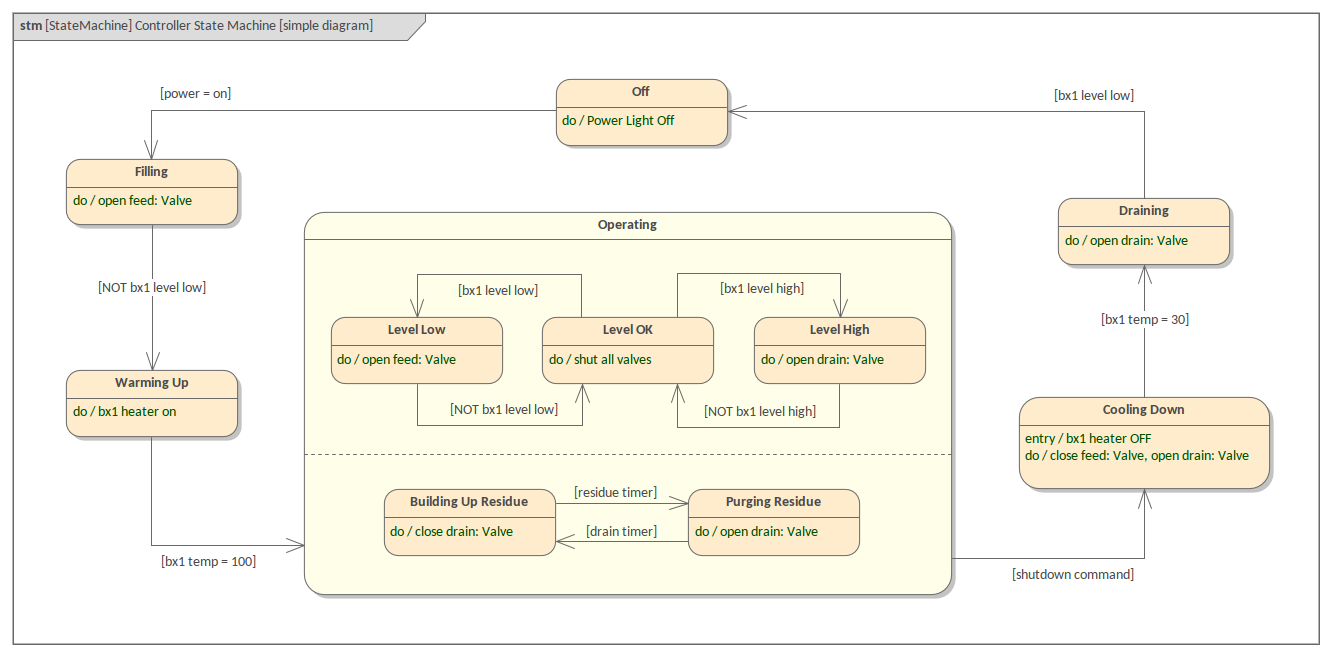
\includegraphics[width=67mm, keepaspectratio]{figures/sysml_state_machine.png}\hspace{1cm}
	\caption{A SysML State Machine.}
	\label{fig:sysml_state_machine}
\end{figure}

State Machines can also have \emph{composite} states and regions, which help with simplifying the behaviour model.

Along with actions defined on transitions, states may also have multiple actions associated with them. \emph{entry actions} defines a set of actions to be performed \emph{before} the state becomes the current state, \emph{exit actions} is a set of actions to be performed \emph{after} the state is no longer the current state. On a similar logic, \emph{do actions} is a set of actions to perform \emph{while} the state machine is in the given state. This fact will be address more in depth in \autoref{sec:gal_vs_sysml}. 

\subsection{Activity}

Activities are a high-level abstraction over Petri nets. 

-- simple activity diagram --

\subsubsection*{Elements of SysML Activities}

-- metamodel of activities --

\paragraph{Action}

The specific operation an Action describes can be stated in various ways, usually in JavaScript or plain old English (Opaque action). In JavaScript, the engineer may access and change variables inside the containing object, send signals to connected objects, or just call existing functions.

-- example of action with js --

There are many different kinds of Activity Nodes, which describe different behaviour for guiding tokens through them.

\subsubsection*{SysML Activities as Petri Nets}

In this section, I will introduce the semantics of Activities using Petri nets as formal semantics. Note however, since not all elements in SysML activity diagrams have execution semantics, I will only consider a set of the modeling elements, including basic actions, initial nodes, final nodes, join nodes, fork nodes, merge nodes, decision nodes, pins and object/control flows.\cite{fuml}\cite{https://doi.org/10.1002/sys.21524}

\subsection{Combining Behaviours}

In SysML the behaviours can be combined using the Call Behaviour sintax, which means the semantics here is combined with the called behaviour's semantics. For example, a state machine's state may have a do action, in which a Call Behaviour action is specified. 
%----------------------------------------------------------------------------
\section{Formal Verification}\label{sec:formal_verification}
%----------------------------------------------------------------------------

Formal verification is a method for proving or disproving the correctness of a system with mathematical precision. Correctness is checked with respect to certain properties or specifications given by the user. Model checking is a formal verification technique that explores the behaviour of the given model exhaustively, i.e., all relevant behaviours of the model are analysed.

\begin{figure}[!ht]
	\centering
	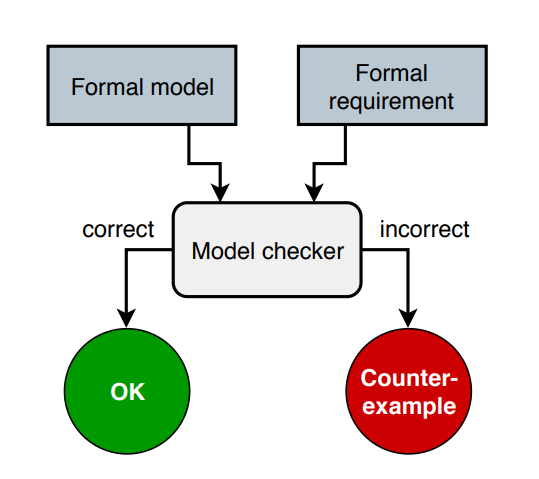
\includegraphics[width=67mm, keepaspectratio]{figures/model_checking.png}\hspace{1cm}
	\caption{An illustration of model checking.}
	\label{fig:model_checking}
\end{figure}

Formal verification tools require the formal model and a formal requirement as input, and return either an ok state, a counter example, or that it can't decide (see \autoref{fig:model_checking}). The counter example is the most important of all, as with its help, the engineers may have a chance of correcting the model.

%----------------------------------------------------------------------------
\section{Extended Symbolic Transition System}\label{sec:xsts}
%----------------------------------------------------------------------------

The high-level nature of engineering models means they are easy-to-use for engineers, but leads to difficulties during the formal verification process. SysML state machines and acitivty diagrams for example contain high-level  constructs that make the modeling workflow more intuitive and enable the modeling of significantly more complex systems, however they are difficult to process using formal methods that are defined on low-level mathematical formalism and verified using SMT solvers. In this section, I introduce the XSTS\cite{xsts} language, which is a low-level modeling formalism designed to bridge the aforementioned gap between engineering models and formal methods.

\subsection{Formal definition}

\begin{definition}[Extended symbolic transition system]
	
	An \emph{Extended symbolic transition system} is a tuple \( XSTS = (D, V, V_C, IV, Tr, In, En) \), where:
	
	\begin{itemize}
		\item \(D = \{ D_{v1}, D_{v2}, \dots, D_{vn} \} \) is a set of value domains;
		\item \(V = \{ v_1, v_2, \dots, v_n \} \) is a set of variables with domains \(D_{v1}, D_{v2}, \dots, D_{vn}\);
		\item \(V_C \subseteq V\) is a set of variables marked as \emph{control variables};
		\item \(IV \in D_{v1} \times D_{v2} \times \dots \times D_{vn}\) is the \emph{initial value function} used to describe the initial state. The initial value function \(IV\) assigns an initial value \(IV(v) \in D_v\) to variables \(v \in V\) of their domain \(D_v\);
		\item \(Tr \subseteq Ops\) is a set of operations, representing the \emph{internal transition relation}; it describes the internal behaviour of the system;
		\item \(In \subseteq Ops\) is a set of operations, representing the \emph{initialisation transition relation}; it is used to describe more complex initialisation, and is executed once and only once, at the very beginning;
		\item \(En \subseteq Ops\) is a set of operations, representing the \emph{environmental transition relation}; it is used to model the system's interactions with its environment.
	\end{itemize}
\end{definition}\label{def:xsts}

In any state of the system a single operation is selected from the sets introduced above (\(Tr\), \(In\) and \(En\)). The set from where the operation can be selected depends on the current state: In the initial state - (which is described by the initialization vector \(IV\)) - only operations from the \(In\) set can be executed. Operations from the \(In\) set can only fire in the initial state and nowhere else. After that, \(En\) and \(Tr\) are selected in an alternating manner.

Operations \(op \in Ops\) describe the transitions between states of the system, where \(Ops\) is the set of all possible transitions. All operations are atomic in the sense that they are either executed in their entirety or none at all. XSTS defines the following operations:

\paragraph{Basic operations}

Basic operations contain no inner (nested) operations. \textbf{Assignments} assign a given value \(v\) from domain \(D_n\) to variable \(V_n\). \textbf{Havocs} behave likewise, except the value is not predetermined; giving a way to assign random value to a variable. Lastly, \textbf{assumptions} check a condition, and can only be executed if their condition evaluates to \emph{true}.

\paragraph{Composite operations}

Composite operations contain other operations, and can be used to describe complex control stuctures. Note that while these are composite operations, their execution is still atomic; meaning that an \emph{assume} operation prevents its containing operations from firing. \textbf{Sequences} are essentially multiple operations executed after each other, while \textbf{parallels} execute all operations at the same time. And lastly, \textbf{choices} model non-deterministic choices between multiple operations; one and only one branch of the choice operation is selected for execution, but that selected operation can still only be executed atomically - e.g., a single failing assume operation can prevent execution.

\subsection{Simple example}

Below is an example XSTS model defined in the language. For a more exact presentation please see \autoref{sec:xsts_language} in the Appendix.

\begin{Verbatim}
	itt majd egy szép xsts példa lesz a running example-re (vagy valami hasonlóra). 
	Akár lehetne egy Gamma által generált statechart is.
\end{Verbatim}


%----------------------------------------------------------------------------
\section{The Gamma Statechart Composition Framework}\label{sec:gamma}
%----------------------------------------------------------------------------

The Gamma Statechart Composition Framework\footnote{https://inf.mit.bme.hu/en/gamma} \cite{mixed_statecharts_2020} is an integrated tool to support the design, verification and validation as well as code generation for component-based reactive systems. The behaviour of each component is captured by a statechart, while assembling the system from components is driven by a domain-specific composition language\footnote{The composition language be the \emph{ibd} model in SysML}. Gamma supports formal verification by mapping composite statecharts to a back-end model checker. Execution traces obtained as witnesses during verification are back-annotated as test cases to replay an error trace or to validate external code generators~\cite{molnar2018gamma}. 

\begin{figure}[!ht]
	\centering
	\includesvg[inkscapelatex=false, width=120mm, keepaspectratio]{gamma-functionality-overview}
	\caption{The overview of model transformation chains and modeling languages of the Gamma framework \cite{mixed_statecharts_2020}. The parts relevant to this work have been marked with red outline.}
	\label{fig:gamma-overview}
\end{figure}

The workflow of Gamma builds on a model transformation chain depicted in \autoref{fig:gamma-overview}, which illustrates the input and output models of these model transformations as well as the languages in which they are defined, and the relations between them. The modeling languages are as follows.

\begin{itemize}
	\item The \textbf{Gamma Statechart Language (GSL)} is a UML/SysML-based statechart language supporting different semantic variants of statecharts.
	\item The \textbf{Gamma Composition Language (GCL)} is a composition language for the formal hierarchical composition of state-based 	components according to multiple execution and interaction semantics.
	\item The \textbf{Gamma Genmodel Language (GGL)} is a configuration language for configuring model transformations.
	\item The \textbf{Gamma Property Language (GPL)} is a property language supporting the definition (CTL*) properties and thus, the formal specification of requirements regarding (composite)	component behavior.
	\item The \textbf{Gamma Trace Language (GTL)} is a high-level specification language for  execution traces of (composite) components.
\end{itemize}

Optionally, statechart models defined in supported modeling tools (front-ends) can be imported into Gamma (Step 1), which can be integrated according to well-defined execution and interaction semantics (Step 2). The resulting composite model is processed and transformed into the input formalisms of integrated model checker back-ends (Step 3). The model checker back-ends provide witnesses (diagnostic traces) based on specified properties, which are back-annotated, resulting in abstract traces (Step 4).
Finally, the abstract traces are mapped into concrete (executable) traces tailored to the targeted execution environment (Step 5). For a more detailed description, see \cite{mixed_statecharts_2020}.

\subsection{Example Statechart}

\autoref{lst:gamma-statechart} shows the Gamma Statechart representation of the State Machine introduced in \autoref{fig:sysml_state_machine}.

\begin{lstlisting}[float,language=statechart, caption={The traffic light controller state machine in the Gamma textual representation.}, label={lst:gamma-statechart}]
package TrafficLightCtrl
import "Interfaces"
statechart TrafficLightCtrl [
	port Control : requires Control
	port PoliceInterrupt : requires PoliceInterrupt
	port LightCommands : provides LightCommands
] {
	timeout BlinkingYellowTimeout3
	timeout BlackTimeout4
	transition from Yellow to Red when Control.toggle
	transition from Normal to Interrupted when PoliceInterrupt.police
	// ...
	transition from BlinkingYellow to Black when timeout BlinkingYellowTimeout3
	transition from Black to BlinkingYellow when timeout BlackTimeout4
	region main_region {
		state Normal {
			region normal {
				shallow history Entry2
				state Green {
					entry / raise LightCommands.displayGreen;
				}
				state Red {
					entry / raise LightCommands.displayRed;
				}
				state Yellow {
					entry / raise LightCommands.displayYellow;
				}
			}
		}
		state Interrupted {
			region interrupted {
				initial Entry1
				state Black {
					entry / set BlackTimeout4 := 500 ms; 
						raise LightCommands.displayNone;
				}
				state BlinkingYellow {
					entry / set BlinkingYellowTimeout3 := 500 ms; 
						raise LightCommands.displayYellow;
				}
			}
		}
		initial Entry0
	}
}
\end{lstlisting}
